\section{Results of the basic part}
\subsection{Correctness}
All indices of the basic part passed all levels of the correctness test.

\subsection{Time complexity}
Figure \ref{fig:BPindextime2}, \ref{fig:BPindextime3}, \ref{fig:BPindextime45} shows the indexing time for Index 2, 3, 4 and 5. Figure \ref{fig:BPindextime2345} shows all indexes compared to each other on a log-transformed plot to compare them against each other.

\begin{figure}[H]
    \centering
     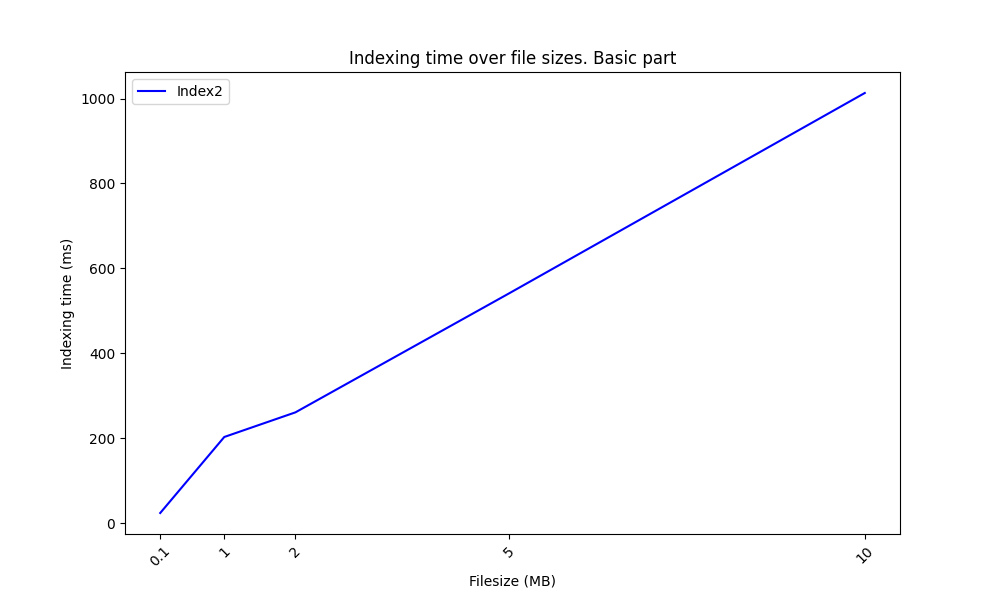
\includegraphics[width=0.7\textwidth]{LaTeX/Pictures/Results/BPIndexing[2].png}
    \caption{Indexing time for Index2 over different file sizes}
    \label{fig:BPindextime2}
\end{figure}

\begin{figure}[H]
    \centering
    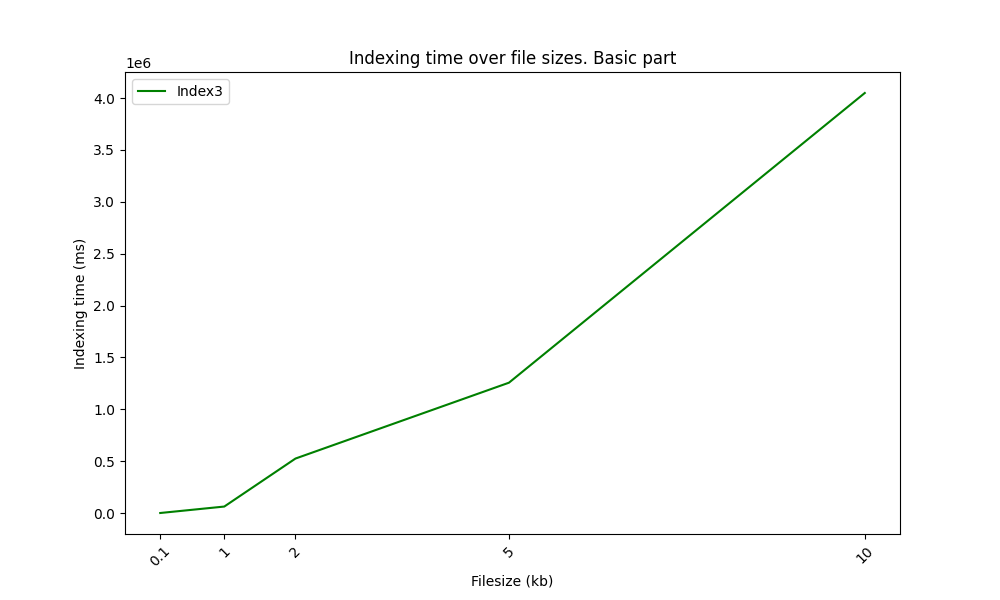
\includegraphics[width=0.7\textwidth]{LaTeX/Pictures/Results/BPIndexing[3].png}
    \caption{Indexing time for Index3 over different file sizes}
    \label{fig:BPindextime3}
\end{figure}

\begin{figure}[H]
    \centering
    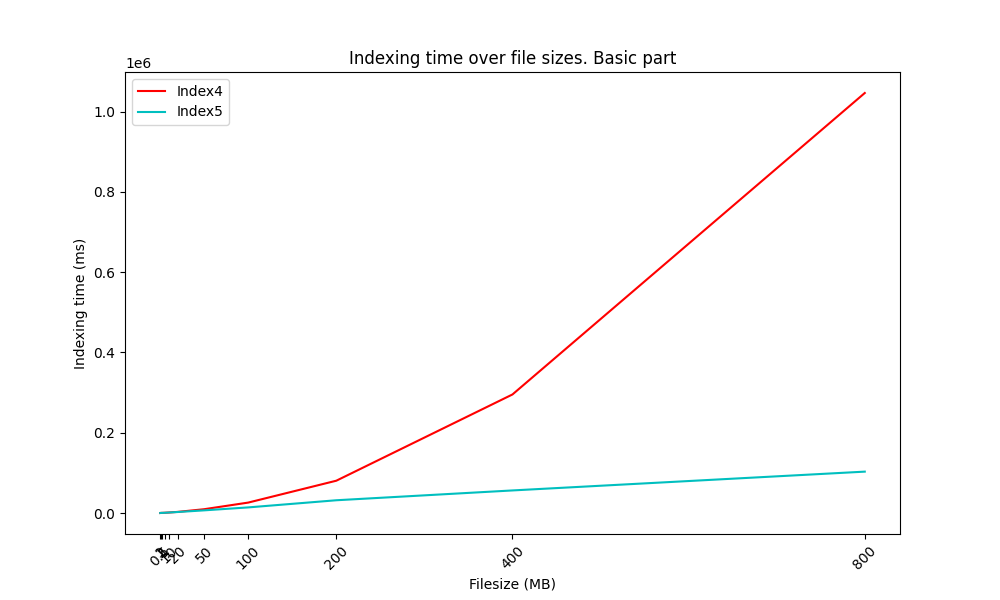
\includegraphics[width=.7\textwidth]{LaTeX/Pictures/Results/BPIndexing[4, 5].png}
    \caption{Indexing time for Index4 and Index5 over different file sizes}
    \label{fig:BPindextime45}
\end{figure}

\begin{figure}[H]
    \centering
    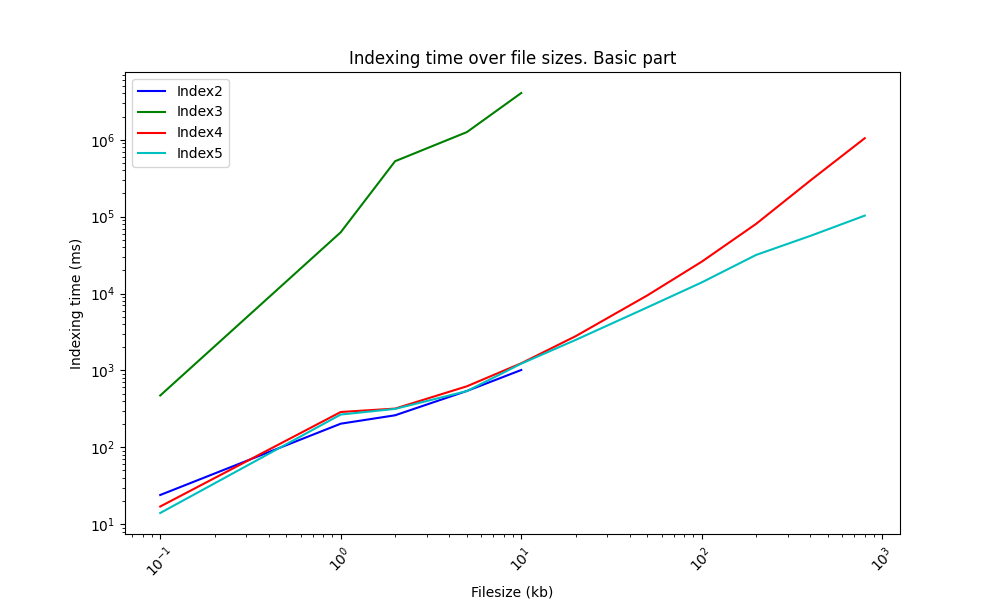
\includegraphics[width=.7\textwidth]{LaTeX/Pictures/Results/BPIndexing[2, 3, 4, 5].png}
    \caption{Indexing time for Index 2,3,4 and 5 over different file sizes.}
    \label{fig:BPindextime2345}
\end{figure}

Figure \ref{fig:BPindextime2} and \ref{fig:BPindextime3}, shows the searching time for Index 2,3,4 and 5.

\begin{figure}[H]
    \centering
    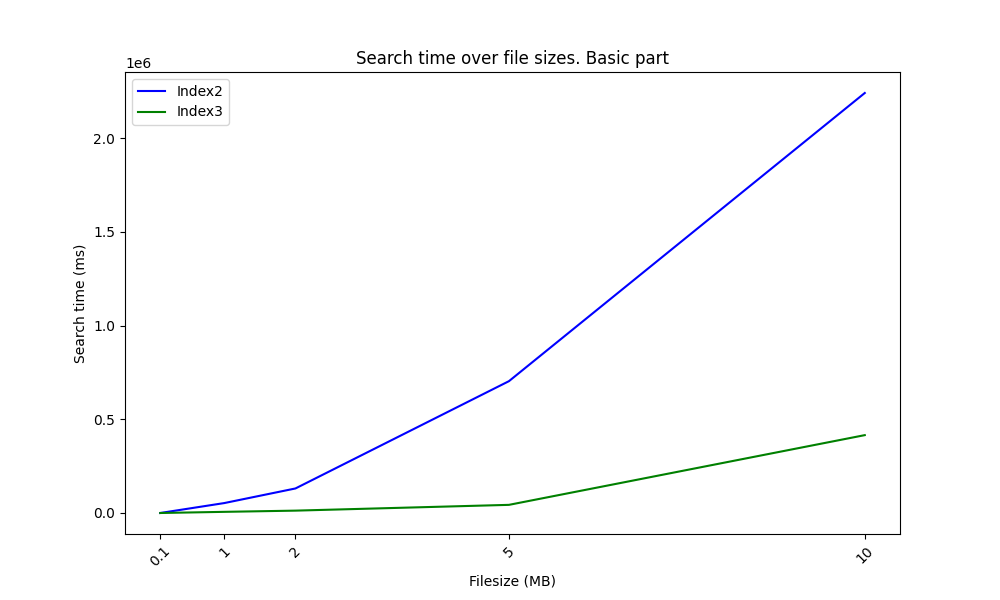
\includegraphics[width=.7\textwidth]{LaTeX/Pictures/Results/BPSearch[2, 3].png}
    \caption{Searching time for searching for all unique words in each file for Index2 and Index3 over different file sizes}
    \label{fig:BPsearch23}
\end{figure}

\begin{figure}[H]
    \centering
    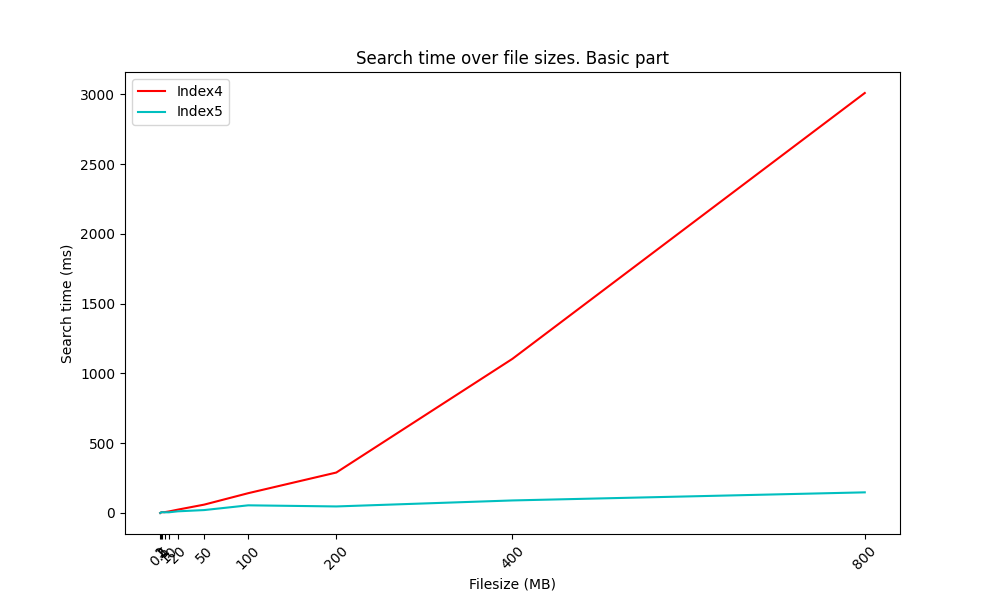
\includegraphics[width=.7\textwidth]{LaTeX/Pictures/Results/BPSearch[4, 5].png}
    \caption{Searching time for searching for all unique words in each file for Index4 and Index5 over different file sizes}
    \label{fig:BPsearch45}
\end{figure} 




